\iffalse 
%%%%%%%%%%%%%%%%%%%%%%%%%%%%%%%%%%%%%%%%%%%%%%%%%%%%%%%%%%%%%%%%%%%%%%%%%%%%%%%%%%%%%%%%
%%%%%%%%%%%%%%%%%%%%%%%%%%%%%%%%%%%%%%%%%%%%%%%%%%%%%%%%%%%%%%%%%%%%%%%%%%%%%%%%%%%%%%%%
%%_______ .___________.    ___      .______    _______                      _____     %%
%%|   ____||           |   /   \     |   _  \  |   ____|                   | ____|    %%
%%|  |__   `---|  |----`  /  ^  \    |  |_)  | |  |__          ______      | |__      %%
%%|   __|      |  |      /  /_\  \   |   ___/  |   __|        |______|     |___ \     %%
%%|  |____     |  |     /  _____  \  |  |      |  |____                     ___) |    %%
%%|_______|    |__|    /__/     \__\ | _|      |_______|                   |____/     %%
%%%%%%%%%%%%%%%%%%%%%%%%%%%%%%%%%%%%%%%%%%%%%%%%%%%%%%%%%%%%%%%%%%%%%%%%%%%%%%%%%%%%%%%%
%%%%%%%%%%%%%%%%%%%%%%%%%%%%%%%%%%%%%%%%%%%%%%%%%%%%%%%%%%%%%%%%%%%%%%%%%%%%%%%%%%%%%%%%
\fi



%%%%%%%%%%%%%%%%%%%%%%%%%%%%%%%%%%%%%%%%%%%%%%%%%%%%%%%%%%%%%%%%%%%
\section{Étape 5: Portage et optimisation du code} \label{sec:methodo_step5}
%%%%%%%%%%%%%%%%%%%%%%%%%%%%%%%%%%%%%%%%%%%%%%%%%%%%%%%%%%%%%%%%%%%
 

%%%%%%%%%%%%%%%%%
\subsection{Motivations et objectifs}
%%%%%%%%%%%%%%%%%


Lors de l'étape 4, une plate-forme a été choisie en fonction de plusieurs critère pour y porter les kernels. L'étape 5 s'occupe du portage du code et de la validation du modèle de performance. Nous montrons comment les outils développés lors de cette thèse sont crucial pour l'analyse de performance. Lorsque le code n'atteint pas les performances espérées, nous proposons un cheminement pour trouver d'où vient ce problème et comment le régler. 


%%%%%%%%%%%%%%%%%
\subsection{Portage de l'application}
%%%%%%%%%%%%%%%%%


\subsubsection{Premier développement}
%%%%%%%%%%%%%%%%%
Une fois la plate-forme choisie il faut appliquer les transformations du code nécessaires pour pouvoir y exécuter les kernels. L'effort nécessaire pour adapter le code à cette nouvelle architecture a dû être évalué lors de l'étape précédente. Le portage du code peut nécessiter un changement de langage de programmation ou de paradigme de programmation.
Si possible, il est important d'utiliser des librairies déjà optimisées pour espérer atteindre les performances crêtes de l'application. De plus, les constructeurs de la plate-forme peuvent avoir développé des librairies (NVIDIA, NEC) pouvant être casi-optimale et qui nécessitent une grande expertise pour être développées.




\subsubsection{Vérification du modèle de performance}
%%%%%%%%%%%%%%%%%

Lors de l'étape 4, un modèle de performance du kernel à été établi (voir paragraphe \ref{sec:smm}). Pour s'assurer des performances du kernel une fois porté, il faut comparer ses performances mesurées avec celles établies par le modèle. Comparer la performance théorique à la performances réelle permet de valider les bonnes performances ou, dans le cas contraire, de les quantifier par rapport à l'optimum théorique $\text{TEMPS}_{optimal}$. Nous avions alors préféré calculer $\text{TEMPS}_{optimal}$ à partir des performances maximales $\text{MEMORY}_{max}$ atteintes par nos benchmark.

Pour mesurer le temps d'exécution du kernel, $\text{TEMPS}_{mesure}$, nous proposons d'utiliser la fonction \textit{gettimeofday ()} \cite{Linux}. Cette fonction est disponible sur la totalité des système linux et permet de récupérer l'heure actuelle avec une précision allant jusqu'à la microseconde. Le but de la méthodologie présentée est de porter les codes sur de nouvelles architectures. Baser l'analyse de performance sur des compteurs matériels trop complexes aurait réduit la portabilité de notre démarche. On peut mesurer  $\text{TEMPS}_{mesure}$ en plaçant deux appels à la fonction \textit{gettime} présentée dans l'\autoref{lst:gettime}, avant et après le kernel.


\begin{lstlisting}[language=c,caption=Fonction utilisée pour lire la date actuelle avec une précision allant jusqu'à la microseconde,label={lst:gettime}, 
  basicstyle=\footnotesize, frame=tb,
  xleftmargin=.065\textwidth, xrightmargin=.065\textwidth]
double gettime()
{
  struct timeval tp;
  struct timezone tzp;
  int i;
  i = gettimeofday(&tp,&tzp);
  return ( (double) tp.tv_sec + (double) tp.tv_usec * 1.e-6 );
}
\end{lstlisting}

Si $\text{TEMPS}_{mesure}$ est proche de $\text{TEMPS}_{optimal}$ alors le kernel est proche d'avoir des performances optimale. En effet, dans le cas de code limité par la bande passante, notre modélisation permet de calculer le temps minimale pour exécuter le kernel, en calculant le temps nécessaire pour déplacer le jeu de données de la mémoire au processeur. Pour un même algorithme il est théoriquement impossible d'exécuter le kernel plus rapidement. La mesure $\text{TEMPS}_{optimal}$ permet d'avoir un objectif de performances à atteindre et de savoir quand le travail d'optimisation est terminé en mesurant simplement son temps d'exécution. Malheureusement, la majorité des applications ont du mal à atteindre cette performance et doivent avoir recourt à des technique d'optimisation de localité pour minimiser le nombre de relecture du jeu de donnée. 




%%%%%%%%%%%%%%%%%
\subsection{Profilage des performances}
%%%%%%%%%%%%%%%%%

Si la mesure de $\text{TEMPS}_{mesure}$  a montrer que le code était inefficace il est alors nécessaire d'en comprendre la raison. Pour cela, le programmeur doit avoir des outils à sa disposition lui permettant de comprendre la cause de ces performances. Même si l'analyse par le modèle du \textit{roofline} a montré que la performance maximale atteignable était limitée par la bande passante mémoire, le proceseur peut lui aussi dégrader les performances (mauvaise compilation, dépendances de données, \textit{cache misses}). Utilisés de façon méthodique les deux outils présentés dans cette thèse, \textit{OProfile++} et \textit{YAMB}, permettent de répondre à beaucoup de question et mener à bien le travail d'optimisation du code dont une vue d'ensemble est proposée sur la \autoref{pic:analyse_bigpicture}.

\begin{figure}
    \center
    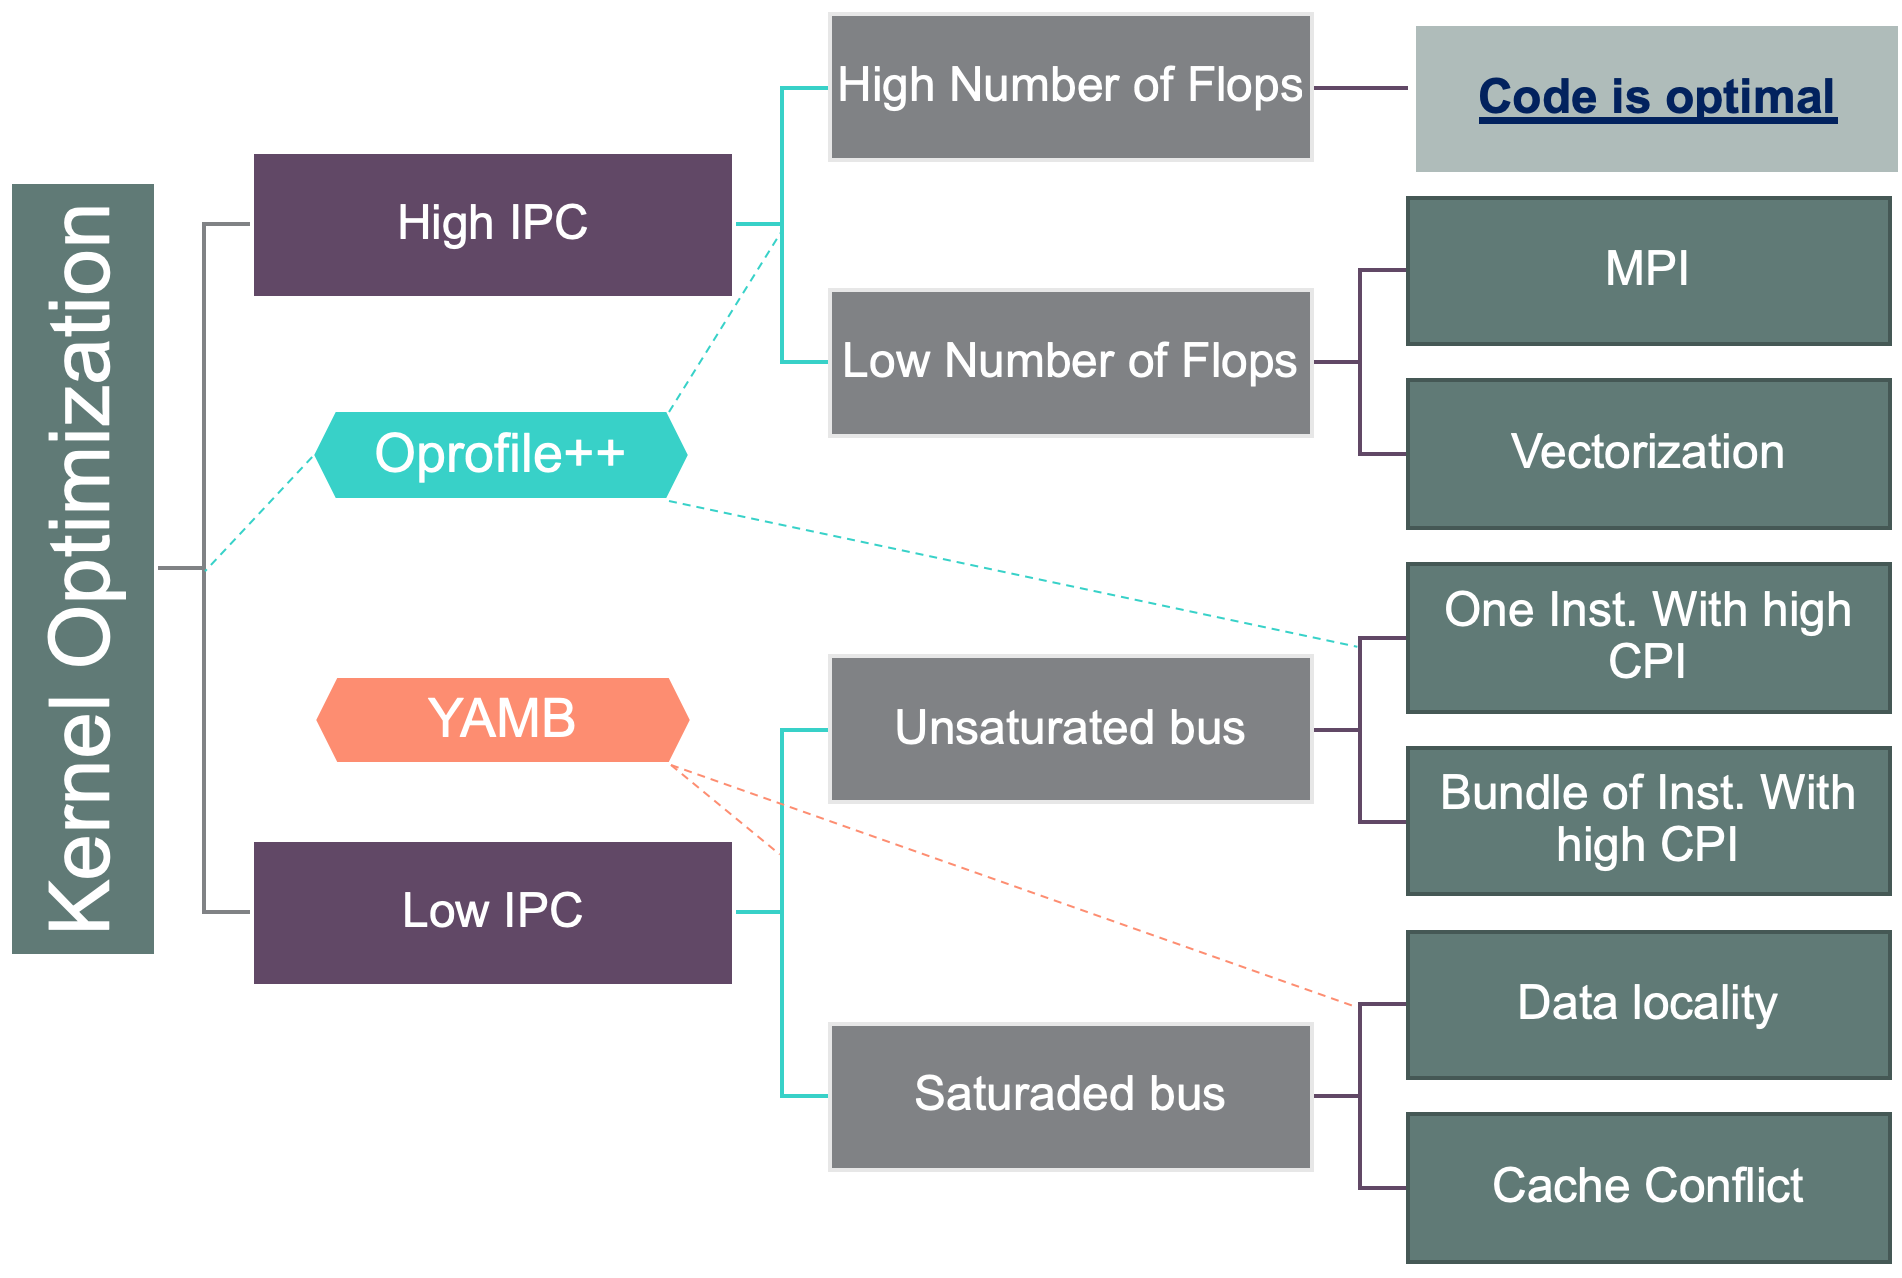
\includegraphics[width=11cm]{images/analyse_bigpicture.png}
    \caption{\label{pic:analyse_bigpicture} Flux de travail pour l'utilisation des outils \textit{Oprofile++} et \textit{YAMB}. La première étape est de mesurer l'IPC du kernel pour déterminer si le processeur ou la mémoire limite les performances. En fonction des observations amenées par les outils, des réponses différentes sont proposées au programmeur pour optimiser son code.}
\end{figure}



\subsubsection{Profilage de la mémoire}
%%%%%%%%%%%%%%%%%
Si la performance est inférieure aux attentes, la première question à se poser est de savoir si le bus mémoire est saturé. Pour y répondre, nous proposons l'outil YAMB qui affiche l'activité du bus mémoire (lecture, écriture et utilisation totale). Pour confirmer sa saturation, il est nécessaire d'avoir caractérisé la performance du bus mémoire dans la première étape. Si le bus n'est pas saturé, la mauvaise performance est due à une autre pathologie. Si le bus est bien saturé et comparer les ratio de lecture/écriture avec ceux mesurée lors de l'étape 3 présentée dans la \autoref{sec:smm}. Grâce à ces ratios, on peut déterminer si le jeu de donnée est lu plusieurs fois, et si des techniques de \textit{blocking} pour améliorer la localité dans la mémoire cache doivent être utilisées. Si le ratio n'est pas celui attendu, c'est parce que le nombre de lectures est plus élevé que prévu. Un mauvais ratio peut provenir d'un nombre de lectures plus élevé que prévu. Ceci est causé par un large éventail de problèmes potentiels, par exemple, des conflits dans le cache, la lecture de données inutiles, une décomposition incorrecte des données ou des structures de mémoire inappropriées. Il est très rare qu'un code écrive plus qu'il ne devrait.





\subsubsection{Profilage du processeur}
L'exécution de l'assembleur peut être suivie avec l'outil \textit{Oprofile++} (voir \autoref{sec:oprofile++}). Il permet d'extraire le code assembleur et d'y agrémenter les compteurs de cycles comme le montre l'\autoref{lst:oprofileex}. L'outil aide pour trouver si des motifs d'instructions sont plus long à exécuter que d'autres, pouvant être expliqué par une dépendance entre les données ou une donnée non présente dans la mémoire cache au moment requis. 
Si des instructions de calculs flottant sont responsables d'un grand nombre de cycle, on peut vérifier le bon fonctionnement du processeurs pour celles ci grâce au générateur de kernels (\autoref{sec:kg}). 


\begin{lstlisting}[language={},caption=L'outil \textit{Oprofile++} permet d'extraire le code assembleur et d'y associer le compteur de cycle,label={lst:oprofileex}, 
  frame=tb]
================================================================
Analysis from the app name (horner1_long) hot spot from the symbole name (f1(double)) which takes 50.1878% 
================================================================
CYCLES       INSTS      ADDRESS    disassembly
----------------------------------------------------------------
     5           11      401be0    vmovupd 0xd1b8(%rip),%ymm1
    39           79      401bf0    vfnmadd231pd 0xd1c7(%rip),%ymm11,%ymm1
     3           14      401bf9    vfmadd213pd %ymm2,%ymm11,%ymm1
...
   760         1652      401c3e    cmp    %eax,%edx
    48           99      401c40    jb     401be0 <_Z8range_f1ddi+0xa0>
----------------------------------------------------------------
LOOP from 401c40 to 401be0  size= 96 sum(cycles)= 2287 
     IPC= 2.12462 cycles/LOOP= 10.3548 flop/cycle = 1.42 
----------------------------------------------------------------
\end{lstlisting}





%%%%%%%%%%%%%%%%%
\subsection{Optimisations: méthodologie d'analyse et d'optimisation}
%%%%%%%%%%%%%%%%%

\textbf{TODO: } écrire une section sur comment optimiser un code en suivant toutes les branches de la figure, et en proposant des optimisations

\begin{figure}
    \center
    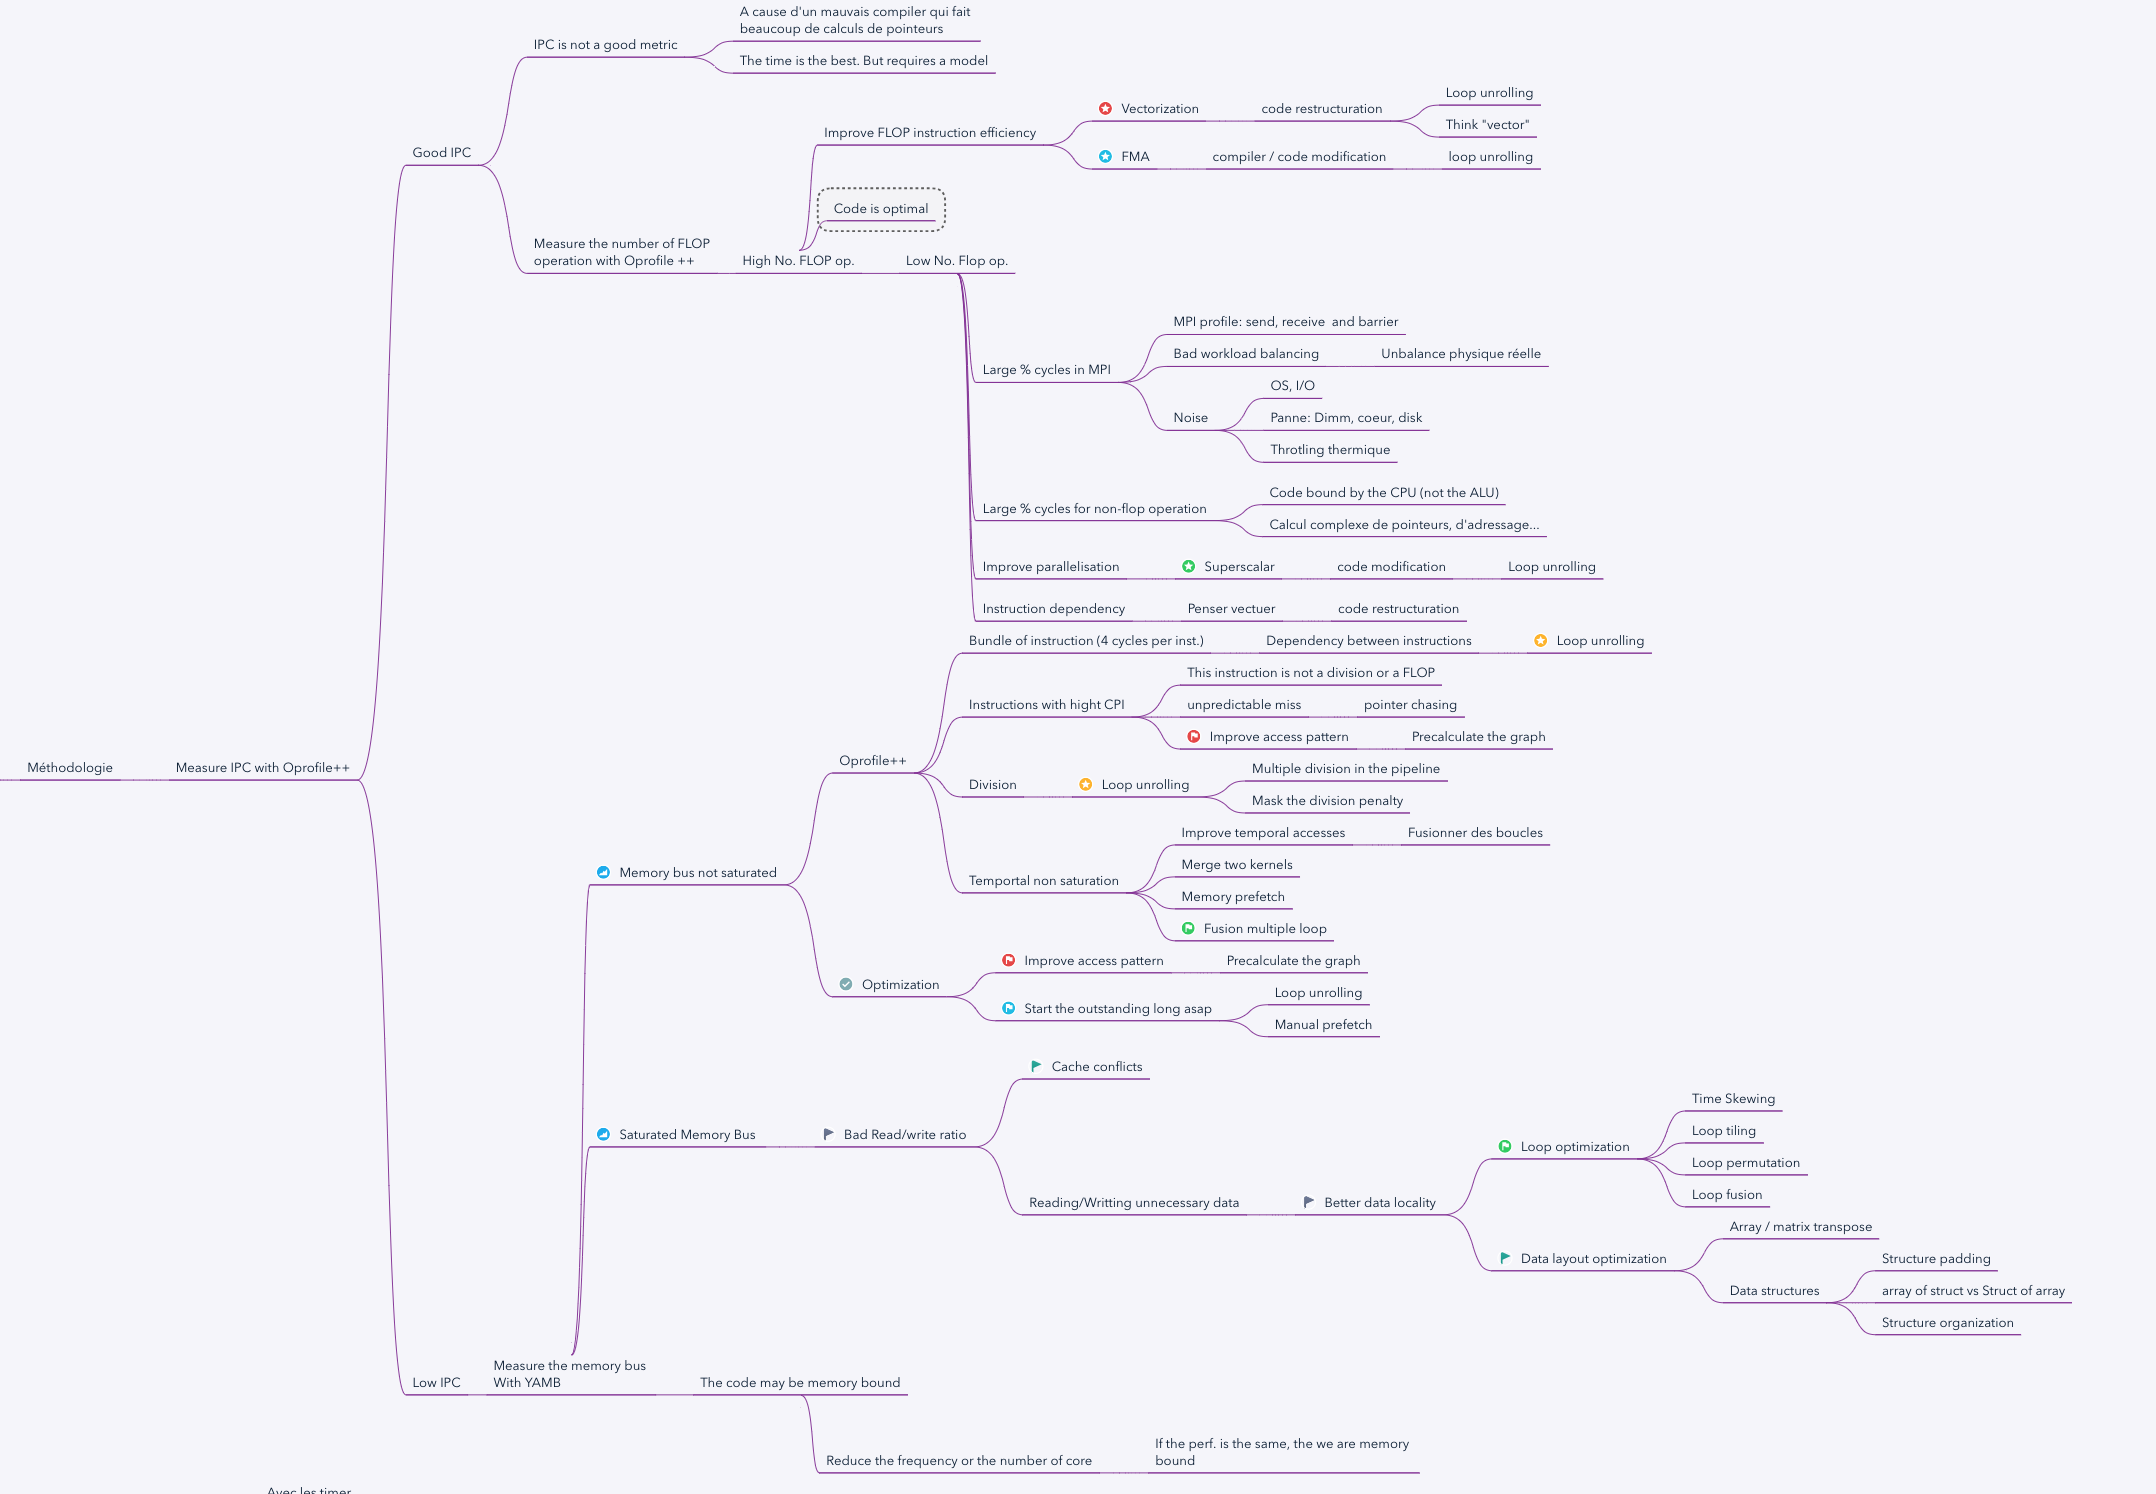
\includegraphics[width=18cm]{images/methodologie_optimisation.png}
    \caption{\label{pic:methodologie_optimisation} \textbf{TODO: } écrire une section sur comment optimiser un code en suivant toutes les branches de la figure, et en proposant des optimisations}
\end{figure}



%%%%%%%%%%%%%%%%%
\subsection{Application au benchmark \textit{Stream}}
%%%%%%%%%%%%%%%%%

Nous appliquons notre méthodologie sur le benchmark Stream fonctionnant sur un processeur Intel Skylake. Cet exercice nous permet de montrer que même sur un code aussi simple, apparemment optimal, notre analyse nous permet de comprendre sa performance et de l'optimiser.


\subsubsection{Vérification du modèle SMM}
%%%%%%%%%%%%%%%%%

Nous avons montré précédemment que la performance du code était limité par la bande passante mémoire. Nous avons appliqué notre modèle de performance SMM et déterminé $\text{TEMPS}_{optimal} = \frac{58.8}{128} = 0.56$ seconde. En utilisant la fonction présenté dans l'\autoref{lst:gettime} nous mesurons $\text{TEMPS}_{mesure} = 0.79$ seconde.

L'application n'est donc pas optimale. Ceci est également validé par le résultat du benchmark Stream qui annonce une bande passante mémoire de 80,13 Go/sec. Pour comprendre ce résultat, nous avons utilisé YAMB pour vérifier que le bus mémoire était bien saturé. Le graphique de la \autoref{fig:stream_before} nous montre que le bus mémoire est utilisé au maximum de son potentiel de 104 GB/s. La saturation du bus n'est donc pas la cause de la mauvaise performance du noyau. Il est alors nécessaire de regarder les rapports lecture/écriture. La \autoref{fig:stream_before} montre cette répartition : 26 Go/s en écriture pour 78 Go/s en lecture, puis un total de 104 Go/s, ce qui correspond à un ratio de 1 écriture pour 3 lectures. Bien que nous nous attendions à un ratio d'une écriture pour deux lectures, ce ratio exact d'une écriture pour trois lectures n'est pas une coïncidence. Un vecteur entier est lu alors qu'il ne devrait pas l'être.

\begin{figure}[htb]
{
\centering
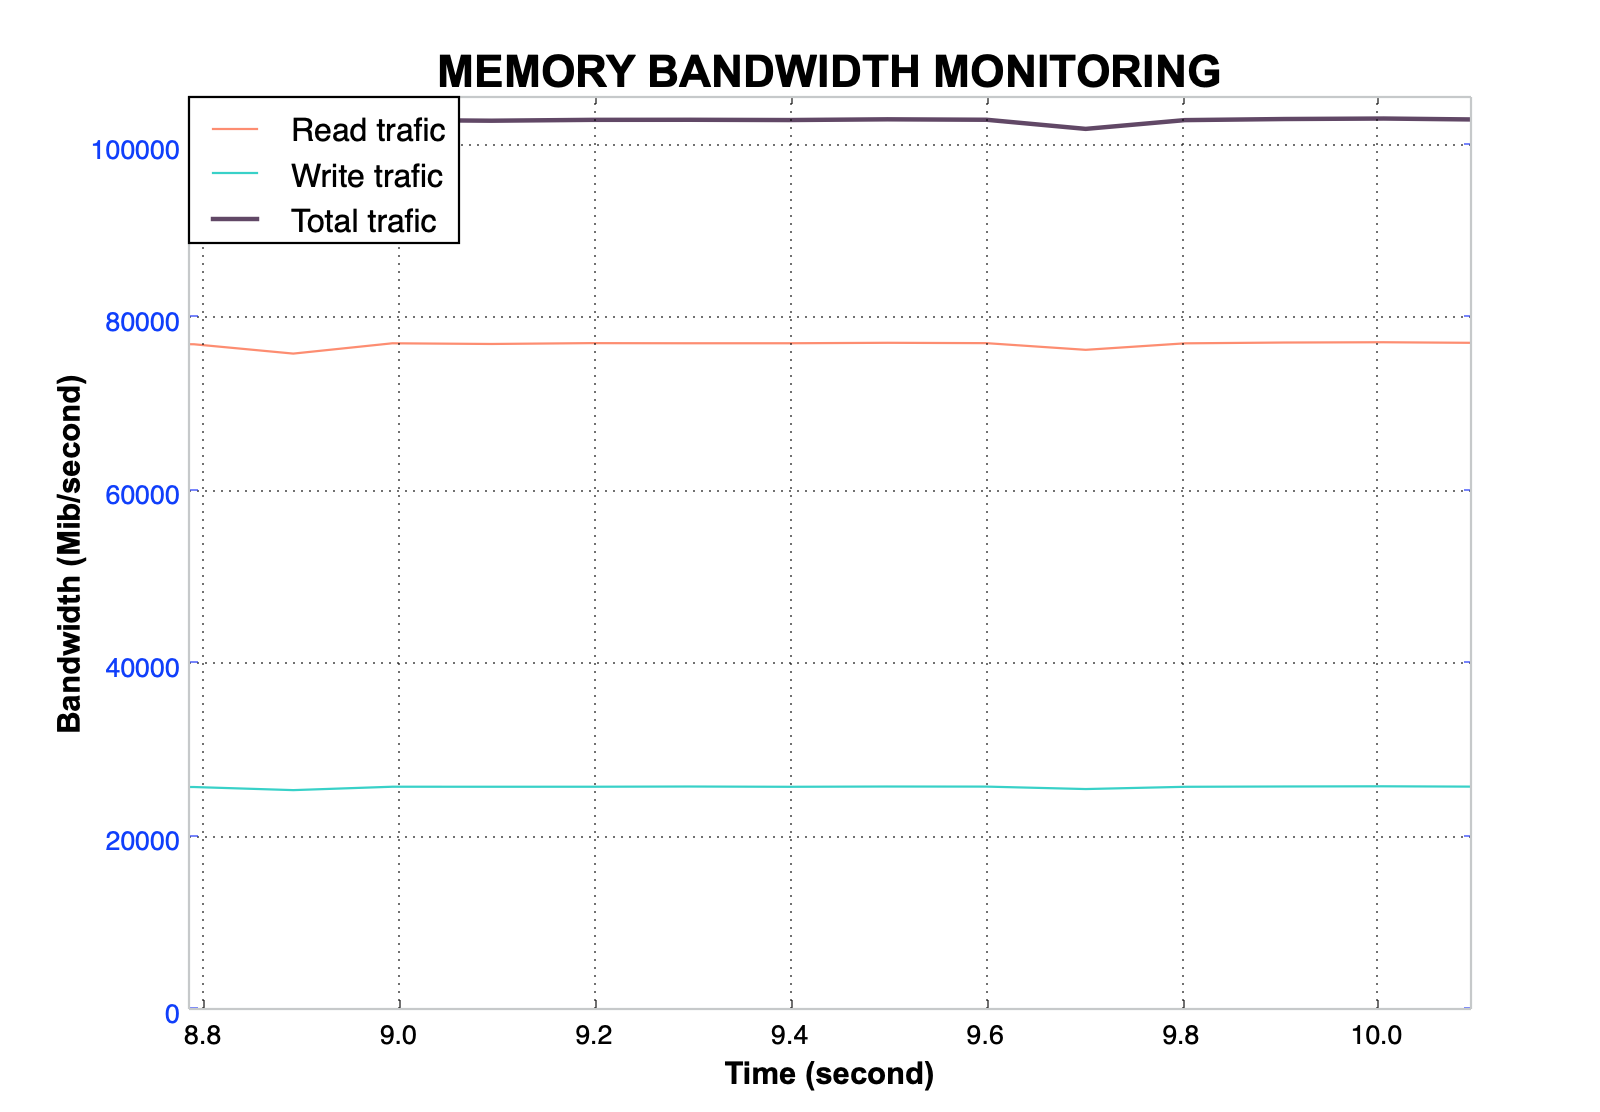
\includegraphics[width=0.80\textwidth]{images/stream_before.png}
\caption{Prolie mémoire donné par l'outil YAMB pour plusieurs exécution de kernel \textit{triadd} du benchmark \textit{Stream}. }\label{fig:stream_before}
}
\end{figure}



\subsubsection{Optimisation du kernel \textit{triadd}}
%%%%%%%%%%%%%%%%%

Les deux vecteurs B et C doivent nécessairement être rouges une fois. La lecture supplémentaire provient du vecteur en écriture A. Ce comportement est dû au processeur qui, avant d'écrire une donnée, charge la ligne de cache correspondante pour la mettre à jour. Cependant, le kernel étudié a la particularité d'écrire toute la ligne de cache, les données initialement présentes n'ayant aucune valeur utile. Une option peut être utilisée avec le compilateur Intel (ICC) pour contourner ce comportement : \textit{-qopt- streaming-stores=always}. Cette option permet au CPU d'écrire toute la ligne de cache sans avoir à la charger.


\subsubsection{Performance du kernel optimisé}
%%%%%%%%%%%%%%%%%

Nous avons compilé \textit{Stream} avec l'option \textit{-qopt- streaming-stores=always} et mesuré le temps et la bande passante de la même manière que pour la première exécution. Les résultats sont résumés dans le \autoref{table:stream_res}. Le temps passé dans le noyau est de 0,59 seconde, beaucoup plus proche du maximum théorique de 0,56 seconde. En analysant la bande passante mémoire, on constate que le rapport lecture/écriture est maintenant de 2 pour 1, les données échangées étant de 34 Go/s en mode écriture pour 68 Go/s en mode lecture. Le total approche la limite du bus, maintenant 102GB/s.

 \renewcommand{\arraystretch}{1.2}
    \setlength{\tabcolsep}{8pt}
    
    \begin{table}[htbp]
        \centering

        \caption{Performance du kernel \textit{triadd} du benchmark \textit{Stream} avant et après optimisation. Le temps (seconde) après optimisation est proche de l'optimum théorique $\text{TEMPS}_{optimal}$  calculé à 0,56 sec. L'utilisation du bus mémoire est approximativement la même entre les deux versions du code (104 et 102 Go/s). L'option de compilation optimise le rapport lecture/écriture (Go/s) et améliore les performances du code de 25\%.}

            \begin{tabular}{l|c|c|c|c|c|}
            \cline{2-6}
                                            & $\text{T}_{mesure} (s)$ & Stream  (GB/s) & $\text{YAMB}_{read}$ (GB/s) & $\text{YAMB}_{write}$ (GB/s) & $\text{YAMB}_{total}$ (GB/s) \\ \hline
            \multicolumn{1}{|l|}{Orig.}  & 0.79   & 80.13  & 26        & 78         & 104        \\ \hline
            \multicolumn{1}{|l|}{Opti.} & 0.59   & 101.84 & 34        & 68         & 102        \\ \hline
            \end{tabular}
            \label{table:stream_res}
        \end{table}